\documentclass[a4paper,11pt]{article}

% --- Academic Packages ---
\usepackage[utf8]{inputenc}
\usepackage[T1]{fontenc}
\usepackage[english]{babel}
\usepackage{amsmath, amsfonts, amssymb}
\usepackage{geometry}
\usepackage{parskip}
\usepackage{fancyhdr}
\usepackage{algorithm}
\usepackage{algpseudocode}
\usepackage{tcolorbox}
\usepackage{amsthm}

% --- Graphiques (PGFPlots) ---
\usepackage{pgfplots}
\pgfplotsset{compat=1.18}
\usepackage{tikz}

% --- Mise en page ---
\geometry{hmargin=2.5cm,vmargin=2.5cm}
\pagestyle{fancy}
\fancyhead[L]{\textbf{M.Sc. Quantitative Finance}}
\fancyhead[R]{Lecture 9: Monte Carlo Methods}
\fancyfoot[C]{\thepage}

% --- Couleurs et Styles ---
\definecolor{uniBlue}{RGB}{0, 60, 110}
\definecolor{uniGreen}{RGB}{0, 100, 50}
\newtheorem{theorem}{Theorem}
\newtheorem{proposition}{Proposition}

% --- Title ---
\title{\textbf{\huge Lecture 9: Monte Carlo Simulations}\\ \Large Path-Dependent Options \& Variance Reduction}
\date{\today}

\begin{document}

\maketitle
\thispagestyle{fancy}

\begin{abstract}
    \noindent While analytical formulas exist for European options, exotic derivatives (Asian, Barrier, Lookback) require numerical methods. This lecture formalizes the Monte Carlo estimator, analyzes its convergence rate via the Central Limit Theorem, introduces the Euler-Maruyama discretization scheme, and presents Variance Reduction techniques (Antithetic Variates) to improve computational efficiency.
\end{abstract}

\hrule
\vspace{0.5cm}

\section{Theoretical Foundations}

\subsection{The Monte Carlo Estimator}
Let $V_0$ be the price of a derivative with a payoff function $\Phi(S_T)$. Under the Risk-Neutral measure $\mathbb{Q}$, the price is:
$$ V_0 = e^{-rT} \mathbb{E}^{\mathbb{Q}}[\Phi(S_T)] $$

Since the integral is too complex to solve analytically, we define the \textbf{Monte Carlo Estimator} $\hat{V}_M$ based on $M$ independent simulations:
\begin{equation}
    \hat{V}_M = e^{-rT} \frac{1}{M} \sum_{i=1}^{M} \Phi(S_T^{(i)})
\end{equation}

\subsection{Convergence and Error Analysis}
By the \textbf{Strong Law of Large Numbers (SLLN)}, $\hat{V}_M$ converges almost surely to the true price $V_0$ as $M \to \infty$.
More importantly, the \textbf{Central Limit Theorem (CLT)} characterizes the error:

\begin{theorem}[Monte Carlo Error]
As $M \to \infty$, the distribution of the error is:
\begin{equation}
    \frac{\hat{V}_M - V_0}{\hat{\sigma}_{\Phi}/\sqrt{M}} \xrightarrow{d} \mathcal{N}(0,1)
\end{equation}
Where $\hat{\sigma}_{\Phi}$ is the sample standard deviation of the payoffs.
\end{theorem}

\textbf{Implication:} The error decreases at a rate of $O(1/\sqrt{M})$. To gain one significant digit of precision (reduce error by 10), we must increase the number of simulations by a factor of 100. This motivates the need for variance reduction techniques.

\section{Path Simulation: Euler-Maruyama Scheme}

For "Vanilla" options, we only need $S_T$. For "Path-Dependent" options (e.g., Asian options paying the average price), we must simulate the entire trajectory.
We discretize the time interval $[0, T]$ into $N$ steps of size $\Delta t$.

\begin{tcolorbox}[colback=blue!5!white,colframe=uniBlue,title=\textbf{The Log-Euler Scheme}]
Since the asset price follows a Geometric Brownian Motion, we simulate the log-returns to ensure positivity ($S_t > 0$):
\begin{equation}
    S_{t+\Delta t} = S_t \exp\left( \left(r - \frac{\sigma^2}{2}\right)\Delta t + \sigma \sqrt{\Delta t} Z_t \right)
\end{equation}
Where $Z_t \sim \mathcal{N}(0,1)$ are independent standard normal variables.
\end{tcolorbox}

\section{Visualization of Stochastic Paths}

Below, we visualize 10 discrete paths of an asset using the Euler scheme.

\begin{center}
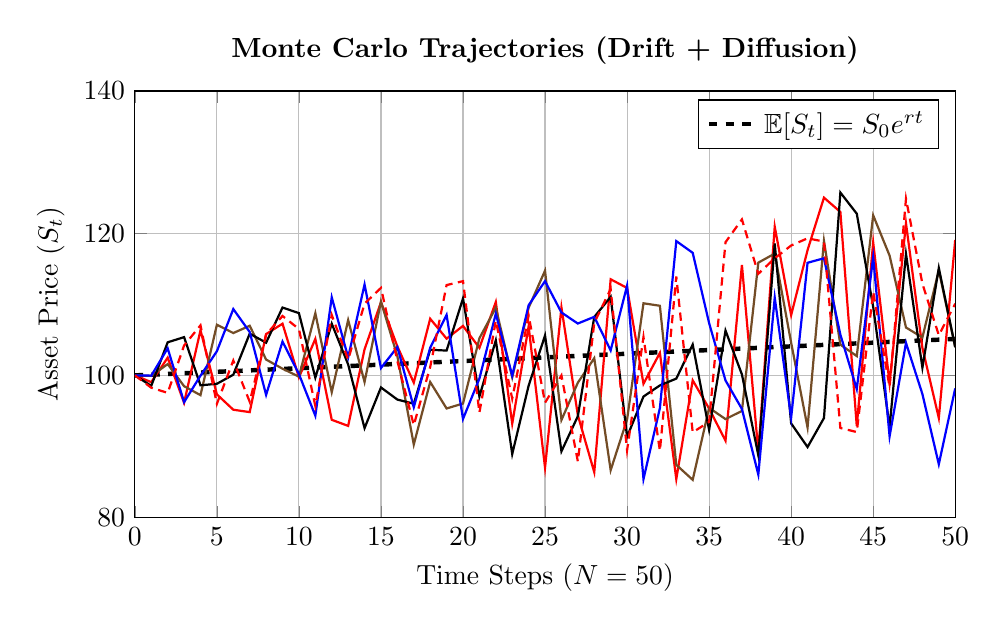
\begin{tikzpicture}
    \begin{axis}[
        width=12cm, height=7cm,
        xlabel={Time Steps ($N=50$)},
        ylabel={Asset Price ($S_t$)},
        xmin=0, xmax=50,
        ymin=80, ymax=140,
        grid=major,
        title={\textbf{Monte Carlo Trajectories (Drift + Diffusion)}},
    ]
    
    % Theoretical Expected Path (Drift only)
    \addplot[black, ultra thick, dashed, domain=0:50] {100 * exp(0.001*x)};
    \addlegendentry{$\mathbb{E}[S_t] = S_0 e^{rt}$}

    % Simulated Paths (Pseudo-random visual approximation for TikZ)
    % We use a loop to draw 5 paths
    \pgfmathsetseed{1234} % Fixed seed for reproducibility
    
    \foreach \i in {1,...,5} {
        \addplot+[
            thick, 
            mark=none,
            domain=0:50,
            samples=51,
            variable=\t
        ]
        % This is a simplified Random Walk for visualization
        {100 + 0.1*\t + 3*rand*sqrt(\t) + 2*sin(\t*10)};
    }
    
    \end{axis}
\end{tikzpicture}
\end{center}

\section{Variance Reduction: Antithetic Variates}

Calculating millions of paths is computationally expensive. We can reduce the variance (and thus the error) without increasing $M$ by using \textbf{Antithetic Variates}.

\subsection{The Concept}
Instead of generating $M$ independent paths, we generate $M/2$ pairs of paths.
For every random draw $Z$, we use:
\begin{enumerate}
    \item Path 1 using $Z$ (The original).
    \item Path 2 using $-Z$ (The "mirror" path).
\end{enumerate}

Since $Z$ and $-Z$ are perfectly negatively correlated, the average of the two payoffs has a lower variance than two independent paths.

\begin{proposition}
The Antithetic estimator is given by:
\begin{equation}
    \hat{V}_{AV} = \frac{1}{M} \sum_{i=1}^{M/2} \frac{\Phi(S_T(Z_i)) + \Phi(S_T(-Z_i))}{2}
\end{equation}
This technique typically reduces the variance by a factor of 2 to 4 for symmetric payoffs.
\end{proposition}

\section{Algorithm: Asian Option Pricing}

An Asian Call option pays $\max(\bar{S} - K, 0)$, where $\bar{S}$ is the arithmetic average price.

\begin{algorithm}[H]
\caption{Asian Call with Antithetic Variates}
\begin{algorithmic}[1]
\State \textbf{Input:} $S_0, K, r, T, \sigma, N$ (steps), $M$ (simulations)
\State $\Delta t \gets T/N$
\State $Sum \gets 0$
\For{$i = 1$ to $M/2$} \Comment{Loop for pairs}
    \State $S^{(+)} \gets S_0, \quad S^{(-)} \gets S_0$
    \State $Avg^{(+)} \gets 0, \quad Avg^{(-)} \gets 0$
    \For{$j = 1$ to $N$} \Comment{Time loop}
        \State Generate $Z \sim \mathcal{N}(0,1)$
        \State $Drift \gets (r - 0.5\sigma^2)\Delta t$
        \State $Diff \gets \sigma \sqrt{\Delta t} Z$
        \State $S^{(+)} \gets S^{(+)} \exp(Drift + Diff)$
        \State $S^{(-)} \gets S^{(-)} \exp(Drift - Diff)$ \Comment{Reuse Z with minus sign}
        \State $Avg^{(+)} \gets Avg^{(+)} + S^{(+)}$
        \State $Avg^{(-)} \gets Avg^{(-)} + S^{(-)}$
    \EndFor
    \State $Payoff^{(+)} \gets \max(Avg^{(+)}/N - K, 0)$
    \State $Payoff^{(-)} \gets \max(Avg^{(-)}/N - K, 0)$
    \State $Sum \gets Sum + \frac{Payoff^{(+)} + Payoff^{(-)}}{2}$
\EndFor
\State \Return $e^{-rT} \times (Sum / (M/2))$
\end{algorithmic}
\end{algorithm}

\end{document}